\documentclass[12pt]{article}
\usepackage[utf8]{inputenc}
\usepackage{amsmath,amsfonts,amssymb}
\usepackage{bm}
\usepackage{graphicx}
\usepackage{enumerate}
\usepackage{listings}
\usepackage{biblatex}
\usepackage[colorlinks,citecolor=blue,urlcolor=blue,bookmarks=false,hypertexnames=true]{hyperref}
\addbibresource{sources.bib}
\usepackage[svgnames]{xcolor}    
\usepackage{indentfirst} 


\usepackage{setspace} 

\onehalfspacing
\pagenumbering{roman} 

\usepackage[top=2cm,bottom=2cm,left=3cm,right=3cm,marginparwidth=1.75cm]{geometry}

\lstset{language=R,
	basicstyle=\scriptsize\ttfamily,
	commentstyle=\color{DarkGreen},
	frame=single,  
}

\newtheorem{theorem}{Theorem}[section]
\newtheorem{corollary}{Corollary}[theorem]
\newtheorem{lemma}[theorem]{Lemma}
\newtheorem{proposition}{Proposition}
\newtheorem{definition}{Definition}

\begin{document}
	\begin{definition}
		\label{definition:f_and_phi}
		Let $f: \mathbb{R}^2 \rightarrow \mathbb{R}$ and $\Phi: \mathbb{R}^2 \rightarrow graph(f) \subseteq \mathbb{R}^3$ where $\Phi(x, y) = (x, y, f(x, y)))$ and both $f$ is a smooth functions. $\Phi$ is invertible where $\Phi^{-1}: graph(f) \rightarrow \mathbb{R}^2$ and $\Phi^{-1}(x, y, f(x, y)) = (x, y)$.
	\end{definition}
	
	\begin{proposition}
		\label{proposition:f_and_phi_smooth_inf_diff}
		Because $f$ is smooth, $\Phi$ is also smooth. Consequently, they are both infinitely differentiable.
	\end{proposition}
	
	
	\begin{definition}
		\label{definition:length_euclidean}
		Let $\sigma: [0, 1] \rightarrow graph(f) \subseteq \mathbb{R}^3$ with $\sigma(t) = (\sigma_1(t), \sigma_2(t), \sigma_3(t))$. The length of this curve $l(\sigma)$ in Euclidean space is given by:
		
		\begin{align}
			l(\sigma) &= \int_{0}^{1} \sqrt{\sigma_1^2(t) + \sigma_2^2(t) + \sigma_3^2(t)} ~ dt\\
			&= \int_{0}^{1} \sqrt{\sigma^{\prime}(t) \cdot \sigma^{\prime}(t) } ~ dt 
			\label{length_euclidean}
		\end{align}
	\end{definition}
	
	\begin{proposition}
		\label{proposition:length_non_euclidean}
		Let $\gamma: [0, 1] \rightarrow \mathbb{R}^2$ and set $\sigma = \Phi \circ \gamma$. From  definition \ref{definition:length_euclidean}, the length of $\sigma(t)$ under the transformation is:
		
		\begin{align}
			\label{equation:length_non_euclidean}
			l_{\Phi}(\sigma) &= \int_{0}^{1} \sqrt{(\Phi \circ \gamma)^{\prime}(t) \cdot (\Phi \circ \gamma)^{\prime}(t)} ~ dt
		\end{align}
	\end{proposition}
	
	\begin{definition}
		\label{defintion:inner_product}
		For two vectors in $\mathbb{R}^2$, $\bm{u} = (u_1, u_2)$ and $\bm{v} = (v_1, v_2)$, the dot product is $\bm{u} \cdot \bm{v} = u_1v_1 + u_2v_2$. However, we will need to use a more general form, the inner product to account for the transformation to the space. The inner product $\langle \bm{u}, \bm{v} \rangle$ must satisfy the following conditions:
		
		\begin{enumerate} [i]
			\item $\langle ~.~,~.~ \rangle: \mathbb{R}^2 \times \mathbb{R}^2 \rightarrow \mathbb{R}$
			\item $\langle \bm{u}, \bm{u} \rangle \geq 0 ~\text{and}~ \langle \bm{u}, \bm{u} \rangle = 0 \iff \bm{u} = 0$
			\item $\langle \alpha(\bm{u} + \bm{w}), \bm{w} \rangle = \alpha \langle \bm{u}, \bm{w} \rangle + \alpha \langle \bm{u}, \bm{w} \rangle$
			\item $\langle \bm{u}, \bm{v} \rangle = \langle \bm{v}, \bm{u} \rangle$
		\end{enumerate}
		
		\noindent Let $\bm{e_1} = (1, 0)$ and $\bm{e_2} = (0, 1)$ be our base vectors in $\mathbb{R}^2$ and $\langle \bm{u}, \bm{v}\rangle$ is as follows:
		
		\begin{align}
			\langle \bm{u}, \bm{v}\rangle &= u_1v_1(\bm{e_1} \cdot \bm{e_1}) + u_1v_2(\bm{e_1} \cdot \bm{e_2}) + u_2v_1(\bm{e_2} \cdot \bm{e_1}) + u_2v_2(\bm{e_2} \cdot \bm{e_2}) \\ 
			&= (u_1, u_2)
			\begin{pmatrix}
				\label{equation:inner_product_identity}
				\bm{e_1} \cdot \bm{e_1} & \bm{e_1} \cdot \bm{e_2} \\
				\bm{e_2} \cdot \bm{e_1} & \bm{e_2} \cdot \bm{e_2} 
			\end{pmatrix}
			\begin{pmatrix}
				v_1 \\ v_2
			\end{pmatrix} \\
			&= (u_1, u_2) \begin{pmatrix}
				1 & 0 \\
				0 & 1 
			\end{pmatrix}
			\begin{pmatrix}
				v_1 \\ v_2
			\end{pmatrix} \\
			&= \bm{u}^{\intercal}\mathbb{I}\bm{v}
		\end{align}
	\end{definition}
	
	\noindent Note that in euclidean space, $\bm{e_1} \cdot \bm{e_2} = \bm{e_2} \cdot \bm{e_1} = 0$ and so $\langle \bm{u}, \bm{v}\rangle = u_1v_1 + u_2v_2$ which is the dot product. Our inner product is now formed such that we can derive a matrix $\bm{A}$ from base vectors of our transformed space. 
	
	\begin{definition}
		\label{defintion:A_matrix}
		Let $\bm{A}$ be a 2x2 real, symmetric and positive definite matrix such that $\bm{A}: \mathbb{R}^2 \rightarrow Matrices(\mathbb{R}^2)$. 
	\end{definition}
	
	\begin{definition}
		\label{definition:inner_product_a_matrix}
		Our inner product in a non-euclidean space transformed at any point $(x, y)$ by $f$ is given by $\langle \bm{u}, \bm{v} \rangle _f(x, y) = \bm{u}^{\intercal}\bm{A}_f(x, y)\bm{v}$.
	\end{definition}
	
	\noindent Our claim is that the expression used to calculate the length of $\gamma(t)$ in non-euclidean space (equation \ref{equation:length_non_euclidean}) can be expressed as an inner product (definition \ref{definition:inner_product_a_matrix}) containing the matrix $\bm{A}$. More formally:
	
	\begin{equation}
		\label{equation:claim}
		(\Phi \circ \gamma)^{\prime}(t) \cdot (\Phi \circ \gamma)^{\prime}(t) = \langle \dot \gamma(t), \dot \gamma(t) \rangle_f(\dot \gamma(t)) =  \dot \gamma(t) \bm{A}_f(\dot \gamma(t)) \dot \gamma(t)
	\end{equation}
	
	\begin{proposition}
		\label{proposition:a_matrix_calc}
		The matrix $\bm{A}$ that satisfies equation \ref{equation:claim} is the following:
		
		\begin{align}
			\bm{A}_f(x, y) = \begin{pmatrix}
				1 + \frac{\partial f}{\partial x}(x, y)^2 & \frac{\partial f}{\partial x}(x, y)^2\frac{\partial f}{\partial y}(x, y) \\
				\frac{\partial f}{\partial x}(x, y)\frac{\partial f}{\partial y}(x, y)   & 1 + \frac{\partial f}{\partial y}(x, y)^2
			\end{pmatrix}
		\end{align}
		
		\noindent Proof: Let $v_1^{(x, y)}(t) = t\bm{e_1} + (x, y)$ and $v_2^{(x, y)}(t) = t\bm{e_2} + (x, y)$ be our base vector functions. These functions are chosen such that $\dot v_1^{(x, y)}(t) = \bm{e_1}$ and $\dot v_2^{(x, y)}(t) = \bm{e_2}$. Our formulation of the inner product in equation \ref{equation:inner_product_identity} gives some indication on how our $\bm{A}$ matrix will be formed. If we compose $\Phi$ with our base vector functions then we can extract a function which provides the base vectors of the transformed space at any point $(x, y)$. This composition for $v_1^{(x, y)}(t)$ and $v_2^{(x, y)}(t)$ is $(\Phi \circ v_1^{(x, y)})^{\prime}(0)$ and $(\Phi \circ v_2^{(x, y)})^{\prime}(0)$ respectively. And, from this we can define our $\bm{A}$ matrix:
		
		\begin{align}
			\centering
			\bm{A}(x, y) = \begin{pmatrix}
				(\Phi \circ v_1^{(x, y)})^{\prime}(0) \cdot (\Phi \circ v_1^{(x, y)})^{\prime}(0) & (\Phi \circ v_1^{(x, y)})^{\prime}(0) \cdot (\Phi \circ v_2^{(x, y)})^{\prime}(0) \\
				(\Phi \circ v_2^{(x, y)})^{\prime}(0) \cdot (\Phi \circ v_1^{(x, y)})^{\prime}(0) & (\Phi \circ v_2^{(x, y)})^{\prime}(0) \cdot (\Phi \circ v_2^{(x, y)})^{\prime}(0)
			\end{pmatrix}
		\end{align}
		
		\noindent Now we need to evaluate each of these expressions. Firstly, we can simplify $v_1$ and $v_2$ as $v_1^{(x, y)}(t) = (t + x, y)$ and $v_2^{(x, y)}(t) = (x, y + t)$ respectively. We will look at $v_1$ since the derivation is similar to that of $v_2$.  
		\begin{align}
			(\Phi \circ v_1^{(x, y)})^{\prime}(0) &= (t + x, y, f(t + x, y))^{\prime}(0) \\
			&= (1, 0, \frac{d}{dt}f(t + x. y))(0)
		\end{align}
		
		\noindent And given that by the chain rule:
		\begin{align}
			\frac{d}{dt}f(x(t), y(t)) &= f_x(x(t), y(t))\dot x(t) + f_y(x(t), y(t))\dot y(t)
		\end{align}
		
		\noindent The expression becomes:
		\begin{align}
			(\Phi \circ v_1^{(x, y)})^{\prime}(0) &= (1, 0, \frac{\partial f}{\partial x}(x, y))
		\end{align}
		
		\noindent And when we evaluate the dot product, our entry for row 1 column 1 of the $\bm{A}$ matrix becomes:
		
		\begin{align}
			(\Phi \circ v_1^{(x, y)})^{\prime}(0) \cdot (\Phi \circ v_1^{(x, y)})^{\prime}(0) &=  (1, 0, \frac{\partial f}{\partial x}(x, y)) \cdot (1, 0, \frac{\partial f}{\partial x}(x, y)) \\ &= 1 + \frac{\partial f}{\partial x}(x, y)^2
		\end{align}
		
		\begin{figure}
			\centering
			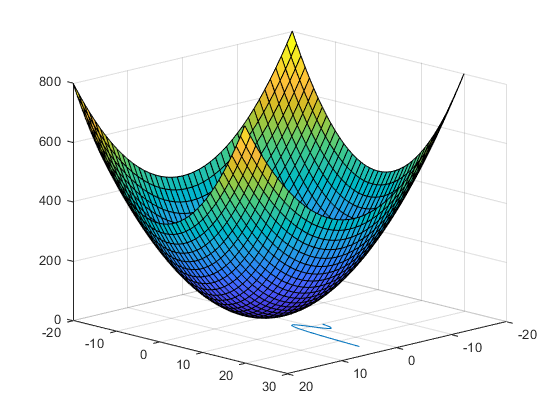
\includegraphics[scale = 0.6]{mapping.png}
			\caption{A random curve in blue and the mapping function $f(x, y) = x^2 + y^2$.}
			\label{fig:mapping function}
		\end{figure}
		
		\noindent Similar calculations will yield the other entries in the table, verifying proposition \ref{proposition:a_matrix_calc}.
	\end{proposition}
	
	\begin{lemma}
		\label{lemma:claim_LHS}
		The following equation is true:
		\begin{align}
			(\Phi \circ \gamma)^{\prime}(t) \cdot (\Phi \circ \gamma)^{\prime}(t) = \dot \sigma^{2}_1(t) + \dot \sigma^{2}_2(t) + (\frac{\partial}{\partial x}f(\sigma(t))\dot \sigma_1(t) + \frac{\partial}{\partial y}f(\sigma(t))\dot \sigma_2(t))^2
		\end{align}
		Proof:
		\begin{align}
			(\Phi \circ \gamma)(t) &= (\sigma_1(t), \sigma_2(t), f(\sigma(t))) \\
			(\Phi \circ \gamma)^{\prime}(t) &= (\dot \sigma_1(t), \dot \sigma_2(t), \frac{d}{dt}f(\sigma(t))) \\
			&= (\dot \sigma_1(t), \dot \sigma_2(t), \frac{\partial}{\partial x}f(\sigma(t))\dot \sigma_1(t) + \frac{\partial}{\partial y}f(\sigma(t))\dot \sigma_2(t)) \\
			(\Phi \circ \gamma)^{\prime}(t) \cdot (\Phi \circ \gamma)^{\prime}(t) &= \dot \sigma^{2}_1(t) + \dot \sigma^{2}_2(t) + (\frac{\partial}{\partial x}f(\sigma(t))\dot \sigma_1(t) + \frac{\partial}{\partial y}f(\sigma(t))\dot \sigma_2(t))^2
		\end{align}
	\end{lemma}
	
	\begin{proposition}
		We can now prove our claim that $(\Phi \circ \gamma)^{\prime}(t) \cdot (\Phi \circ \gamma)^{\prime}(t) = \dot \gamma(t) \bm{A}_f(\gamma(t)) \dot \gamma(t)$.
	\end{proposition}
	
	
	\vspace{5pt}\noindent\emph{RHS:}
	\begin{align}
		\dot \gamma(t) \bm{A}(\gamma(t)) \dot \gamma(t) &= 
		(\dot \gamma_1(t), \dot \gamma_2(t))      
		\begin{pmatrix}
			1 + \frac{\partial f}{\partial x}(x, y)^2 & \frac{\partial f}{\partial x}(x, y)^2\frac{\partial f}{\partial y}(x, y) \\
			\frac{\partial f}{\partial x}(x, y)\frac{\partial f}{\partial y}(x, y) & 1 + \frac{\partial f}{\partial y}(x, y)^2
		\end{pmatrix}
		\begin{pmatrix}
			\dot \gamma_1(t) \\ \dot \gamma_2(t)
		\end{pmatrix} \\
		&= (\dot \gamma_1(t) + \dot \gamma_1(t) \frac{\partial}{\partial x}f(\gamma)^2 + \dot \gamma_2(t) \frac{\partial}{\partial x}f(\gamma(t))\frac{\partial}{\partial y}f(\gamma(t)), \\ 
		& \dot \gamma_2(t) + \dot \gamma_2(t) \frac{\partial}{\partial x}f(\gamma(t))^2 + \dot \gamma_1(t) \frac{\partial}{\partial x}f(\gamma(t))\frac{\partial}{\partial y}f(\gamma(t)))
		\begin{pmatrix}
			\dot \gamma_1(t) \\ \dot \gamma_2(t)
		\end{pmatrix} \\
		&= \dot \gamma_1(t)^2 + \dot \gamma_1(t)^2 \frac{\partial}{\partial x}f(\gamma(t))^2 + 2\dot \gamma_1(t) \dot \gamma_2(t) \frac{\partial}{\partial x}f(\gamma(t)) \frac{\partial}{\partial y}f(\gamma(t)) \\ &+ \dot \gamma_1(t) \dot \gamma_2(t) + \dot \gamma_2(t)^2 + \dot \gamma_2(t)^2 \frac{\partial}{\partial y}f(\gamma(t))^2 \\
		&=  \dot \gamma^{2}_1(t) + \dot \gamma^{2}_2(t) + (\frac{\partial}{\partial x}f(\gamma_1(t), \gamma_2(t))\dot \gamma_1(t) + \frac{\partial}{\partial y}f(\gamma_1(t), \gamma_2(t))\dot \gamma_2(t))^2
	\end{align}
	
	Which is equivalent to the result derived in lemma \ref{lemma:claim_LHS}. Therefore, our claim that $(\Phi \circ \gamma)^{\prime}(t) \cdot (\Phi \circ \gamma)^{\prime}(t) = \dot \gamma(t) \bm{A}_f(\gamma(t)) \dot \gamma(t)$ is true. From this, we can redefine the non-euclidean length:
	
	\begin{align}
		l(\sigma) &= \int_{0}^{1} \sqrt{\langle \sigma^{\prime}(t), \sigma^{\prime}(t) \rangle _f(x, y)} ~ dt \\ &=  \int_{0}^{1} \sqrt{\sigma^{\prime}(t)\bm{A}_f(\sigma(t))\sigma^{\prime}(t)^\intercal} ~ dt
		\label{non_euclidean_length_expression}
	\end{align}
	
	Lets look at the programmatic implementation of this in the function \break \texttt{utility\_fitness\_non\_euclidean\_3d}. At the beginning, we used the identity matrix for our \texttt{par\$non\_euclidean\_A} parameter. If the curve between two points is a straight line, then this can verify that the implementation is correct. The code below is an interpretation of equation \ref{non_euclidean_length_expression} however we are treating time as discrete rather than continuous. \break
	
	\begin{lstlisting}
# function to calculate non euclidean distance
utility_fitness_non_euclidean_3d <- function(self, genotype, par){ 
	complete_genotype <- rbind(par$non_euclidean_start, genotype, 
							   par$non_euclidean_end);
	
	if (is.null(par$non_euclidean_A)){
		par$non_euclidean_A <- array(c(1, 0, 0, 1), dim = c(2, 2));
	};
	
	bounds <- par$non_euclidean_bounds;
	curve <- complete_genotype;
	
	differential <- differentiate(genotype);
	
	time_interval <- (bounds[2] - bounds[1]) / (dim(curve)[1] - 1);
	time_stamps   <- ((1:dim(curve)[1]) - 1) * time_interval;
	
	differential <- array(append(time_stamps, differential), dim = dim(curve));
	
	total_area <- 0;
	for (time_index in 1:(dim(curve)[1] - 1)){
		current_gradient <- differential[time_index, ];
		A_component <- current_gradient %*% par$non_euclidean_A;
		magnitude   <- sqrt(sum(A_component * current_gradient));
		
		local_area <- magnitude * time_interval;
		total_area <- total_area + local_area;
	}
	return(total_area)
}
	\end{lstlisting}
	
	\begin{figure}[h!]
		\centering
		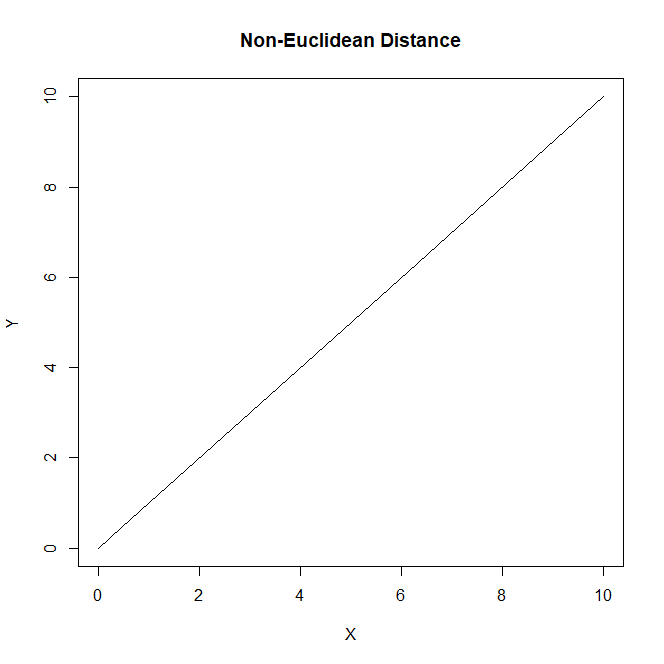
\includegraphics[scale = 0.27]{non-euclidean-distance-const.png}
		\caption{Non-Euclidean Distance: Using an Identity Matrix}
		\label{non-euclidean-const-results}
	\end{figure}
	
	Using the identity matrix as A will result in the curve shown in figure \ref{non-euclidean-const-results}. Because this graph is a straight line, we can now replace our matrix A with a matrix function that changes depending on the location in the space. We will use $f(x, y) = x^2 + y^2$ to define the matrix A:
	
	\begin{align}
		A_f(x, y) = \begin{pmatrix}
			1 + \frac{\partial f}{\partial x}(x, y)^2 & \frac{\partial f}{\partial x}(x, y)^2\frac{\partial f}{\partial y}(x, y) \\
			\frac{\partial f}{\partial x}(x, y)\frac{\partial f}{\partial y}(x, y) & 1 + \frac{\partial f}{\partial y}(x, y)^2
		\end{pmatrix} = \begin{pmatrix}
			1 + 4x^2 & 4xy \\
			4xy & 1 + 4y^2
		\end{pmatrix}
	\end{align}
	
	\begin{lstlisting}
		# calculate the relative A matrix for the function f(x, y) = x^2 + y^2
		get_A <- function(coordinate){
			x <- coordinate[1];
			y <- coordinate[2];
			
			return(array(c(
			1 + (4*(x^2)), 4*x*y, 4*x*y, 1 + (4*(y^2))
			), dim = c(2, 2)))
		}
	\end{lstlisting}
	
	We've replaced the parameter \texttt{par\$non\_euclidean\_A} with the function \texttt{get\_A()} inside of the fitness function, which will return the corresponding matrix A for a given coordinate. The coordinate we are using is the average of the coordinates on each side of the segments which make up the curve. The \texttt{par\$non\_euclidean\_start} and \texttt{par\$non\_euclidean\_end} will be $(0, 10)$ and $(10, 0)$ respectively. You can run this simulation using the \texttt{ga\_example()} function from the ga-package:
	
	\begin{lstlisting}
		# run the non-euclidean-var example
		gapackage::ga_example(name = "non-euclidean-var")
	\end{lstlisting}
	
	The simulation will result in the curve shown in figure \ref{fig:non-euclidean-distance-var}. You can see that it curves around the parabolic shape of the function. I've taken the data for this curve and used MATLAB to plot the curve on the function to make it more clear what is going on. You can see this in figure \ref{fig:mapping_with_second}. The blue line represents the shortest Euclidean distance between the two coordinates. The red line shows the shortest distance between the two coordinates where the space is transformed according the function $f(x, y) = x^2 + y^2$.
	
	\begin{figure}
		\centering
		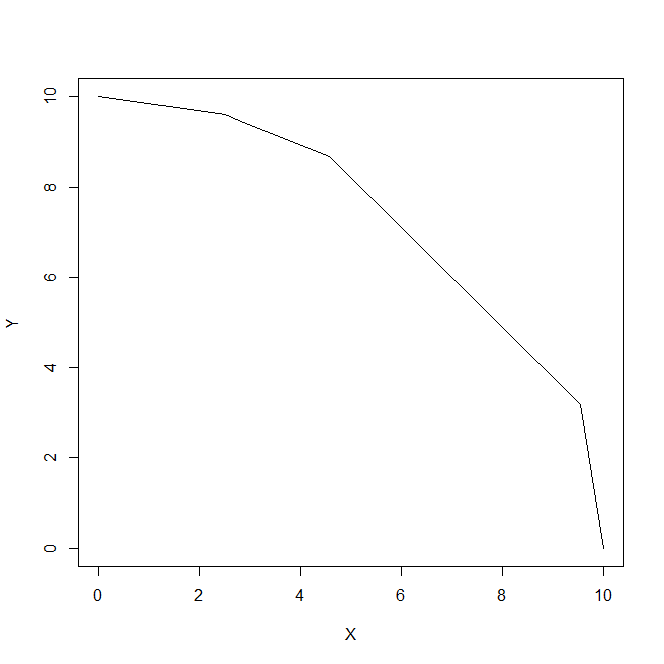
\includegraphics[scale = 0.4]{non-euclidean-distance-var.png}
		\caption{Non-Euclidean Distance: Relative A Matrix Results}
		\label{fig:non-euclidean-distance-var}
	\end{figure}
	
	\begin{figure}
		\centering
		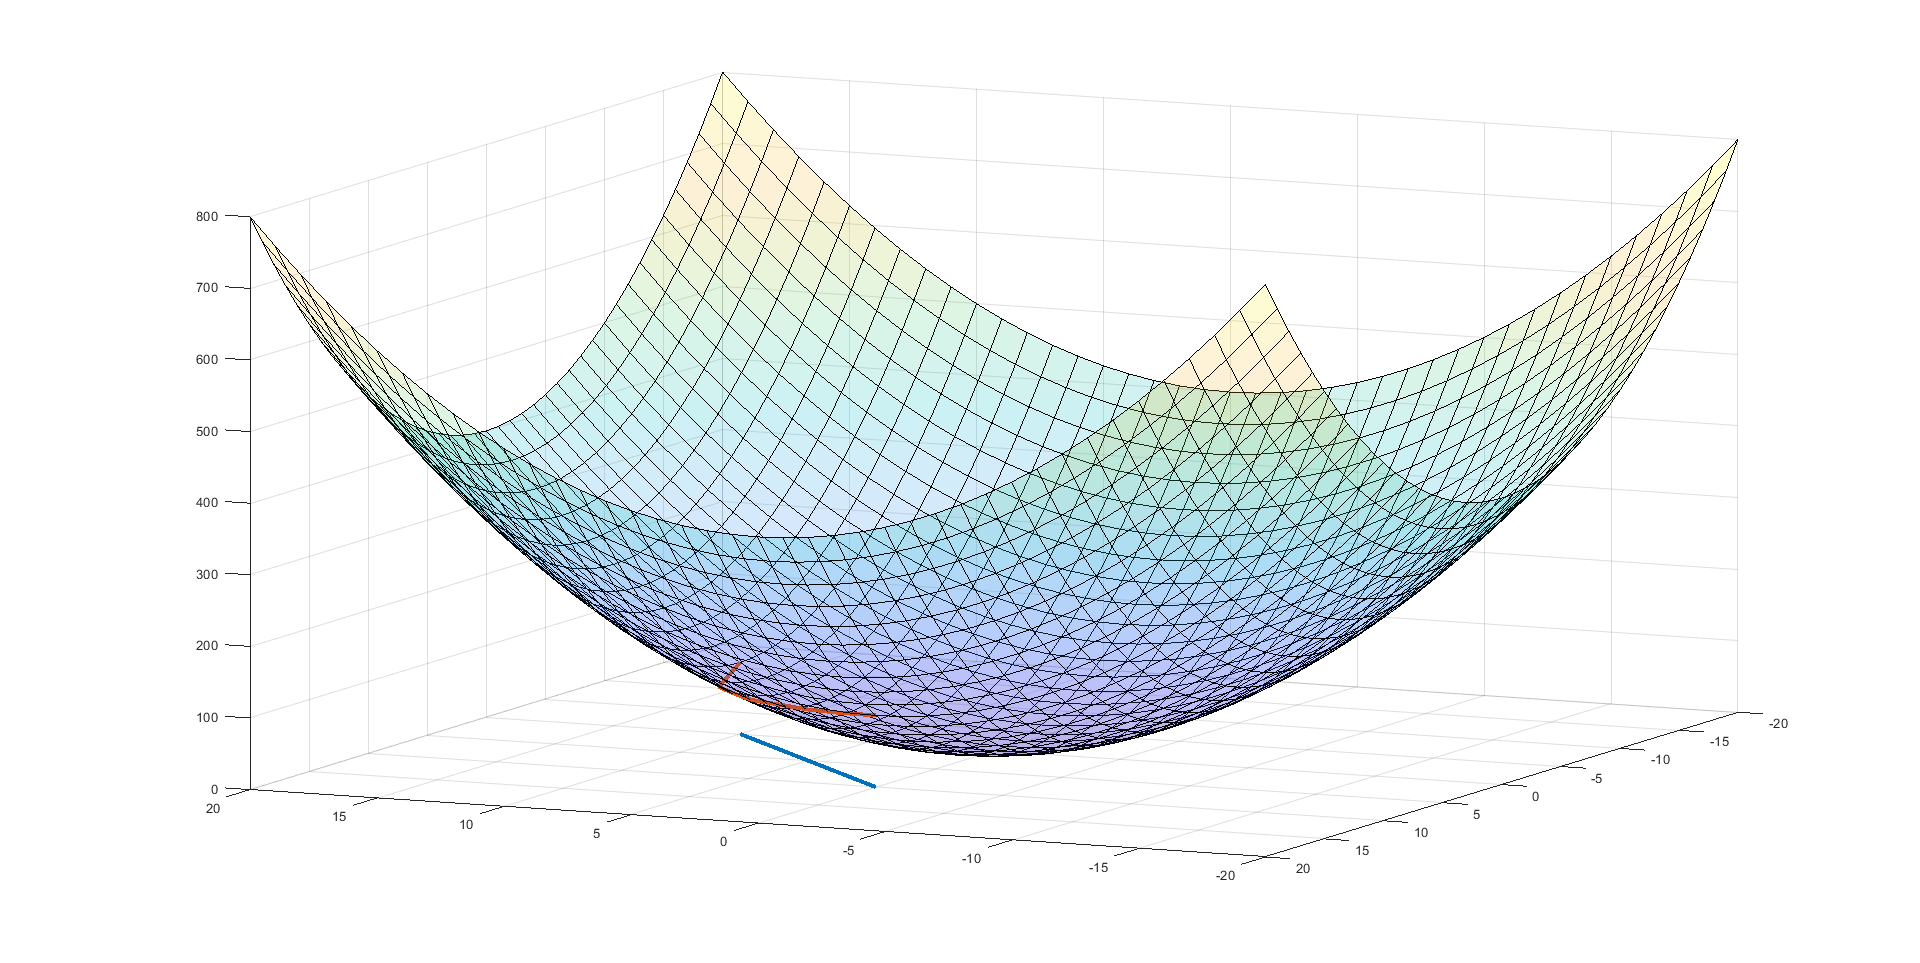
\includegraphics[scale = 0.2]{mapping_with_second.png}
		\caption{Euclidean Distance (Blue) / Non-Euclidean Distance (Red) on Function $f(x, y) = x^2 + y^2$}
		\label{fig:mapping_with_second}
	\end{figure}
\end{document}